\documentclass[review,authoryear,english]{elsarticle}

\usepackage{babel}
\usepackage{natbib}

\bibliographystyle{elsarticle-harv}

\usepackage{lineno}
\usepackage[utf8]{inputenc}  %% Permite utilizar tildes si archivo usa utf-8
\usepackage{amsmath}
\usepackage{amssymb}

\modulolinenumbers[1]

\usepackage{xcolor}
\usepackage{soul}
\usepackage{marginnote}
\usepackage{float}

\definecolor{yellow}{rgb}{1.0,1.0,0.25} %   light yellow
\definecolor{dkred}{rgb}{0.5,0,0}       %   dark red
\definecolor{todocolor}{rgb}{1.0,0.8,0.5}

\usepackage[hidelinks]{hyperref}

\newcommand{\todohdr}{Please review:}

% Crea una caja rojiza aparte
\newcommand{\TODO}[2][\todohdr]{%
\smallbreak\noindent\colorbox{todocolor}{%
\begin{minipage}{1\linewidth}
\textbf{#1}\par{\footnotesize{#2}}
\end{minipage}}}

% crea un par de palabras, la primera tachada, y la segunda normal
\newcommand{\instead}[2]{\textcolor{dkred}{\st{#1}}#2}

% marca un texto con fondo amarillo y crea una nota al pie con comentario
\newcommand{\todofn}[2]{\colorbox{yellow}{#1}\footnote{\color{dkred}#2}}

% solo marca un texto con fondo amarillo
\newcommand{\review}[1]{\colorbox{yellow}{#1}}

% Unifica la escritura de referencias a figuras, por si hay que
% cambiarlas todas de una vez
\newcommand{\figref}[1]{\figurename~\ref{#1}}

%  \usepackage{epstopdf} 
%  \usepackage{epsfig}

\journal{Computers and Electronics in Agriculture}

\usepackage{subcaption}

\begin{document}
  % where to look for graphics
  \graphicspath{{./}{./fig/}}

\begin{frontmatter}

\title{Forecasting the black Sigatoka development rate:\\ 
A comparison of machine learning techniques}

%% Group authors per affiliation:
\author[afiLuisAlex]{Luis-Alexander Calvo-Valverde\fnref{myfootnote}}
\ead{lualcava.sa@gmail.com}
\fntext[myfootnote]{Corresponding author. (506)70104420}

\author[afiCorbana]{Mauricio Guzmán-Quesada}
\author[afiCorbana]{José-Antonio~Guzmán-Alvarez}
\author[afiPablo]{Pablo Alvarado-Moya}

\address[afiLuisAlex]{DOCINADE, Instituto Tecnológico de Costa Rica, 
Computer Research Center, Multidisciplinar program eScience, Cartago, Costa Rica}

\address[afiCorbana]{Dirección de Investigaciones, Corporación Bananera Nacional~S.\,A., Guápiles, Costa Rica}

\address[afiPablo]{DOCINADE, Instituto Tecnológico de Costa Rica, Cartago, Costa Rica}

\begin{abstract}
Pending.
\end{abstract}

\begin{keyword}
Machine learning \sep Black Sigatoka \sep Support vector regression \sep
Banana disease prediction \sep Biological warning system 
\end{keyword}

\end{frontmatter}

\linenumbers

\section{Introduction}

The black Sigatoka disease caused by the fungus \emph{Mycosphaerella
  fijiensis Morelet} is the major pathological problem of banana and
plantain crops in Central America, Panama, Colombia and Ecuador, as well as in
many parts of Africa and Asia \citep{MarinVargas1995}.

This disease attacks the plant leaves producing a rapid deterioration
of the leaf area. It affects the growth and productivity of the plants
due to the impairment of the photosynthetic process.  Furthermore, it
causes a reduction in the quality of the fruit, and promotes premature
ripening of bunches, which is the major cause of product losses
associated with the black Sigatoka.

For these reasons, warning systems have been developed to detect the
disease and monitor its progress.  For instance, the early warning
system developed by \citet{ganry1983} and modified by
\citet{ganry1972} for the control of the yellow Sigatoka in Cameroon,
was later adapted by \citet{Ternesien1985} and \citet{foure1988} for
the black Sigatoka.

This biological warning system is based on weekly observations of the
disease progression on young leaves of the plant.
%
\figref{fig:diseasestages} shows an example of three progressive
stages of the black Sigatoka.
	 
\begin{figure}[ht] 
\centering
\begin{tabular}{c@{\;}c@{\;}c}
  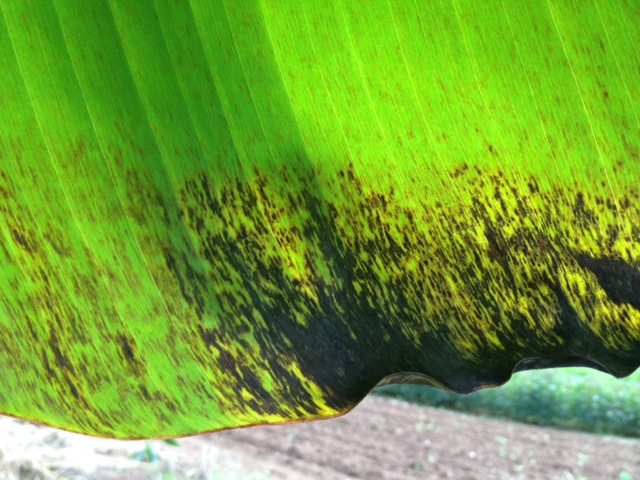
\includegraphics[width=.32\linewidth]{Roya_a} &
  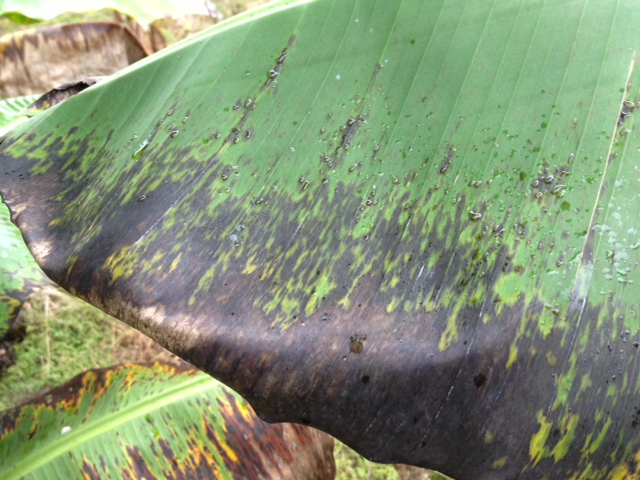
\includegraphics[width=.32\linewidth]{Roya_b} &
  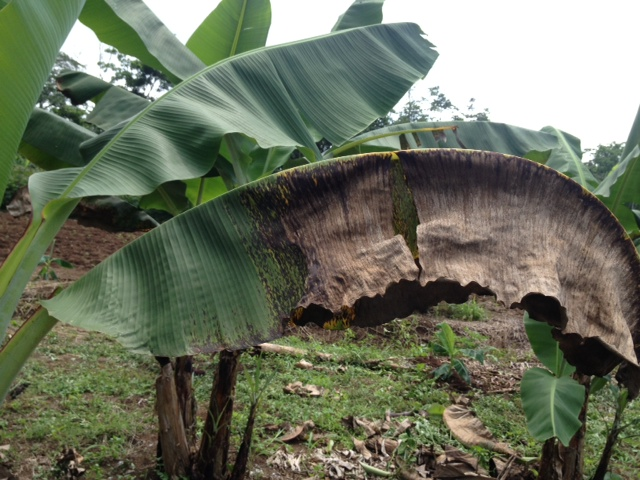
\includegraphics[width=.32\linewidth]{Roya_c} \\
  (a) & (b) & (c) 
\end{tabular}
\caption{Examples of three disease stages of the black Sigatoka. 
(a)~Initial stage. (b)~Intermediate stage, and (c)~Advanced stage.} 
\label{fig:diseasestages} 
\end{figure}

The disease progression is then quantified according to Fouré's scale
of the symptom stages \citep{foure1988} by means of numeric
coefficients that describe the degree of incidence and the severity of
the disease development.  These coefficients are then used to
calculate two variables: gross sum and state of evolution.

The gross sum is based on the present disease progression stage and
the numeric coefficients, which increase with the progression of
the symptoms and the juvenility of the leaf.
%
The state of evolution is calculated using the gross sum and the
foliar emission period.
%
Decades ago threshold levels on these variables were used as a guide
to plan the spray schedules.  Nowadays the fluctuation of these two
variables seems to better suggest appropriate times to spray
\citep{Marinetal2003}.

In Costa Rica the black Sigatoka is frequently treated with
chemical fungicides.
%
Depending on the zone of production and the weather conditions,
45--55~cycles/year of fungicide applications are required to keep this
disease under control and to produce the expected fruit quality for the
international markets.
%
This represents a cost per hectare per year in the range from US\$1600
to US\$2000; about 0.64--0.80 cents of the production costs for a
18.14\,kg box, which overall corresponds to 10\%--12\% of the total
production costs.

The past and present rates of disease development can in principle be
used to predict its future behavior and to determine if a particular
fungicide spray program will be able to effectively treat the disease
in an economically affordable way \citep{ChuangJeger1987}.
%
Phytopathological studies point out that climate has a major effect on
the development of the black Sigatoka, where the main variables
affecting it are precipitation, temperature, relative humidity and
wind \citep{MarinVargas1995}.  Hence, it can be expected that patterns
in these variables correlate with the disease development.

There exist already several efforts to apply machine learning methods
to support decision-making in agriculture, including the control of
crop diseases. For example, \cite{Camargo2012} present an intelligent
system for the assessment of crop disorders, \cite{Huang2010}
introduce a plant virus identification method based on neural networks
with an evolutionary preprocessing stage, \cite{Kim2014} summarize in
their survey crop pests prediction methods using regression and
machine learning approaches, while \cite{Zhao2013} present an
intelligent agricultural forecasting system based on wireless sensor
networks.

\TODO{Importantísimo es explicar aquí brevemente por qué esos otros
  trabajos no se aplican al caso de la Sigatoka, o qué es lo que han
  hecho mal, que este trabajo sí hace bien.}

In this work, we compare five machine learning techniques to predict
the development rate of the black Sigatoka disease: support vector
regression (SVR), echo state networks (ESN), ridge regression,
elastic-net regression and ordinary least squares linear regression,
using input variables such as \review{completar las variables de
  entrada usada} to predict \review{completar las variables de salida}.

\todofn{The main contribution of this work}%
{Definitivamente ese no es el aporte principal del artículo.  Cuando
  esté listo el resto hay que volver aquí.  Creo que va a ser algo
  como mostrar la relevancia de la etapa de preprocesamiento, o
  mostrar que a pesar de ser sistemas complejos, con variables
  caóticas, lo mejor en este caso son predictores lineales, o algo por
  el estilo.} %
% 
 is the selection of the best machine learning technique
to forecast the black Sigatoka development rate according to the
metric indicated below.

The outline of the paper is as follows: Section~\ref{sec:related}
presents related works and Section~\ref{sec:techs} summarizes the
machine learning techniques selected for the analysis. In
Section~\ref{sec:data} we present the methodology used in this study
and describe data used for its verification.  The results and their
discussion are presented in section~\ref{sec:results}.  The
Section~\ref{sec:concl} concludes this article and presents lines for
future works.


\section{Related works}
\label{sec:related}

Several efforts have been made to apply machine learning techniques in
the automated discovery of relationships between environmental
variables and quantified descriptors for variables of agricultural 
interest such as the progress of diseases.
% 
\citet{Huang2010} summarize in their survey the
development of soft computing techniques in agricultural and
biological engineering, including fuzzy logic, artificial neural
networks, genetic algorithms, bayesian inference and decision trees.
%
Similarly, \citet{Kim2014} survey more recent prediction
methods for crop pests using regression and machine learning approaches.

\TODO{Falta indicar qué concluyen los dos surveys anteriores}

In general, the machine learning methods applied to predict the
evolution of plant diseases, can be classified in two main approaches:
1)~those whose main inputs are images, and 2)~Those whose main inputs
are environmental and biological variables. Our study focuses in the
second case.


% %
% For example, 
% 
% Me parece que aquí hay un error: Huang2010 es el survey, y sería mucha
% coincidencia que fuera lo mismo que el \citet{Glezakos2010} ¿o no?
%
% \cite{Huang2010} introduce a plant virus
% identification method based on neural networks with an evolutionary
% preprocessing stage, 
%

\citet{Romero1995} relied on regression models using a stepwise
procedure to predict incubation and disease latency periods for the
black Sigatoka.
% 
He collected environmental data from two different farms in Costa Rica
between December 1993 and August 1995.
%
The prediction models reached coefficients of determination $R^2$ of
69\% or 78\% on the observed data for the incubation and disease
latency periods, respectively; however, the cross validation on
independent data sets failed.

More recently, \citet{Glezakos2010} used genetic algorithms (GA) and
neural networks (NN) to identify the Tobacco Rattle Virus (TRV) and
the Cucumber Green Mottle Mosaic Virus (CGMMV).
%
The method was tested against some of the most commonly used
classifiers in machine learning (Bayes classifiers, decision trees and
$k$-nearest neighbors) via cross-validation and proved their
applicability in these kind of problems.

\citet{Alves2011} used geoinformation techniques to
develop predictive models in the study of risk areas to soybean rust,
coffee leaf rust, and banana black Sigatoka, under consideration of
Brazil’s climatic characteristics and the distribution of soybean,
coffee and banana crops.
%
Temperature and rainfall data were acquired for the period from 1950
to 2000, and simulated data were generated for 2020, 2050 and 2080
using the SRES~A2 climate change scenarios.
%
Using principal components analysis, a single variable was generated
as a linear combination of 57 input variables, in order to determine
an index explaining 87\%, 88\% and 90\% of the
%
\todofn{variability}{variabilidad de qué?}  
%
of soybean, coffee and
banana crops, respectively, in municipal districts across Brazil.
%
The climatic model was used to generate the zoning of the three plant
diseases, using temperature and leaf wetness as input.
%
%Redunda con lo que sigue:
%Areas favorable for the diseases were plotted against the main coffee,
%soybean and banana growing areas in Brazil.
%
This methodology enabled the visualization of the changes in areas
favorable for epidemics under possible future scenarios of climate
change.

Other applications of machine learning methods in precision
agriculture include the use of support vector regression to predict
carcass weight in beef cattle in advance to the slaughter
\citep{Alonso2013}, machine learning assessments of soil drying for
agricultural planning \citep{Coopersmith2014}, and early detection and
classification of plant diseases with support vector machines based on
hyperspectral reflectance \citep{Rumpf2010}.

Furthermore, there have been attempts to generate software
tools. \citet{Camargo2012} presented an information
system for the assessment of plant disorders (Isacrodi).
%
They showed that human experts will attain a much accurate assessment
than the Isacrodi classifier, particularly when provided with samples
from the affected crop. However, in those cases where such expertise
is not available, the authors suggest that Isacrodi can still provide
valuable support to farmers.
%
Isacordi includes 15 crop disorders, but the black Sigatoka is none
of them. The prediction process is based on multi-class support vector
machines.

Regarding the prediction of the black Sigatoka disease development
with machine learning methods, \citet{Bendini2013} presented a study
on the risk analysis of its occurrence based on polynomial models.
%
A case study was developed in a commercial banana plantation located
in Jacupiranga, Brazil. It was monitored weekly from February to
December 2005.
%
The data included the weekly monitoring of the disease’s evolution
stage, time series of meteorological data and remote sensing
data.
%
They obtained a model to estimate the evolution of the disease from
satellite imagery. This model relates gray levels (NC) of the band 2
images of the Landsat-5 satellite, with the progress status or disease
severity (EE). The authors claim to reach an $R^2$ of 90\%.

There are also works related to the banana fruit. \citet{Soares2014}
apply two techniques: artificial neural networks (ANNs) and multiple
linear regression (MLR) in banana plant to predict the yield.
%
Their results show that the neural network is more accurate in
forecasting the weight of the bunch in comparison to the multiple
linear regressors in terms of the mean prediction-error $(MPE =
1.40)$, mean square deviation $(MSD = 2.29)$ and coefficient of
determination $(R^2 = 91\%)$.

% Este no calza, porque no se ve qué es lo de machine learning que usa...
%
%\citet{Zhao2013} present an intelligent agricultural
%forecasting system based on wireless sensor networks.

\TODO{Importantísimo es explicar aquí brevemente por qué esos otros
  trabajos no se aplican al caso de la Sigatoka, o qué es lo que han
  hecho mal, que este trabajo sí hace bien.}

\section{Compared regression techniques}
\label{sec:techs}

In the prediction of the development rate of the black Sigatoka, we
compare techniques such as least squares or ridge regression, commonly
encountered in the agricultural literature with machine learning
methods such as support vector regression, elastic regression and echo
state networks, where the parameter space of each technique is also
taken into account.

\subsection{Ordinary least squares regression}

Given a data set 
\begin{equation}
  D=\left\{(\vct{x}_i,y_i) \mid i=1\ldots n\right\}
\end{equation}
composed of the $d$-dimensional%
\footnote{Without loss of generality assume that the first component
  of every vector $\vct{x}_i$ is always $1$.}
%
feature vectors $\vct{x}_i\in\setR^d$ and the corresponding responses
$y_i$.
%
The ordinary least squares regression (OLSR) fits a linear model
$\tilde{y}_i = f(\vct{x}_i) = \dotp{\vct{w},\vct{x}_i}$ such that the sum of
squares of the residuals $(\tilde{y}_i-y_i)$ is minimized.
%
Let $\mat{X}$ be the $n\times{}d$ feature matrix containing the $i$-th
data sample $\vct{x}_i^T$ in its $i$-th row and $\vct{y}$ contain all
the responses $y_i$ corresponding to each row, then the least squares
regression finds
\begin{equation}
\label{eq:problem}
  \hat{\vct{w}} =
  \arg\min_{\vct{w}} E(\vct{w})
\end{equation}
with the error function
\begin{equation*}
  E(\vct{w}) =  \left\| \mat{X}\vct{w} - \vct{y}\right\|_2^2
\end{equation*}
The solution is found by means of the pseudoinverse
$\hat{\vct{w}}=\mat{X}^+\vct{y}=(\mat{X}^T\mat{X})^{-1}\mat{X}^T\vct{y}$
or equivalently by the singular value decomposition of $\mat{X}$
\citep{Press2007}.

\TODO{Alex, no sé hasta donde hiciste en las pruebas ese ``arreglo''
  de que los datos tengan todos una entrada igual a 1.  De no ser así,
  el método no puede encontrar el offset, y sería como forzar que el
  modelo tenga que pasar por cero...  a menos por supuesto que la
  constante se haya sacado de la ecuación al optimizar...
  
  Comentario:  Pero si por feature scaling los datos están entre -1 y 1, con 0 en medio?}

\subsection{Ridge regression}

In contrast to the OLSR, for the ridge regression (RR)
\citet{Hoerl1988} proposed to add a term to penalize large weights
into the error function
\begin{equation*}
  E(\vct{w}) = 
  \left\| \mat{X}\vct{w} - \vct{y} \right\|_2^2 + 
  \alpha \left\|\vct{w}\right\|_2^2 
\end{equation*}
where the parameter $\alpha>0$ controls how strong is the shrinking of
the estimates towards zero.  This shrinkage introduces some bias but
helps to reduce the variance of the estimate.
%
The solution of the optimization problem (\ref{eq:problem}) in this
case is given by $\hat{\vct{w}}=(\mat{X}^T\mat{X} +
\lambda\mat{I})^{-1}\mat{X}^T \vct{y}$.

\subsection{Elastic net regression}

Instead of $L_2$ regularization prior
($\alpha\left\|\vct{w}\right\|_2^2$) included in the ridge regression,
\citet{Tibshirani1996} used an $L_1$ term ($\lambda
\left\|\vct{w}\right\|_1$) for his lasso estimator, which permits to
select a subset of the available features by zeroing the weights of
the deselected features.
%
If the dimension $d$ of the data is larger than the number $n$ of data
samples, lasso will select a maximum of $d$ variables.

The elastic net regression (ENR) of \citet{Zou2005} combines both
$L_1$ and $L_2$ priors of the ridge and lasso estimators such that the
error function is now
\begin{equation*}
  E(\vct{w}) = 
  \left\| \mat{X}\vct{w} - \vct{y} \right\|_2^2 + 
  \alpha \left\|\vct{w}\right\|_2^2 +
  \lambda \left\|\vct{w}\right\|_1 
\end{equation*}
%
This combination of priors still allows to learn a sparse model with only a 
few weights being non-zero like in the case of lasso, but still
maintaining the regularization properties of the ridge regression
\citep{scikitlearn2011}.

The elastic net is useful when multiple features are correlated: lasso
will likely pick one of these at random, while the elastic net will
still likely pick both.

\TODO{Algo que no entiendo es que las elastic net son en realidad una
  generalización del ridge, Lasso y OLSR.  Así que en los experimentos
  con las selección adecuada de parámetros este método debería
  comportarse al menos igual o mejor que esos otros regresores!  No sé
  hasta donde sea justificable usar este Y los otros, porque este ES
  los otros...
  
  Comentario: En realidad la idea era mostrar los diversos resultados, pero me suena bien reducirlo a ElasticNet (optimizado los parámetros) lo cual reduce resultados y gráficos en dos (quitando ridge y OLSR).  Cuando hablamos confirmamos y lo quito.  }


\TODO{Alex, veo que usas mucho \citep{scikitlearn2011} para los
  métodos, pero ese es solo el paper de un tool y no los proponentes
  originales de los métodos.  Usualmente uno hace referencia a algún
  artículo, libro o tutorial donde ojalá los que propusieron el método
  son los que lo explican.  Ahí metí entonces en las referencias otros
  artículos por ese motivo.
  
  Comentario: muchas gracias..}

\subsection{Support Vector Regression (SVR)}

\TODO{Estoy seguro que los lectores van a solicitar reducir esto y
  dejar solo la referencia.  Dejé solo lo que considero relevante,
  pero podés reducirlo más, si querés.}

From the perspective of Support Vector Regression (SVR) the regression
function is usually formulated as 
\begin{equation}
\label{eq:svrfunc}
  \tilde{y} = f(\vct{x}) = \dotp{\vct{w},\vct{x}} + b
\end{equation}
The weights are selected in a convex optimization problem
\citep{Smola2004}:
\begin{align*}
  \text{minimize} \quad  & \frac{1}{2}\|\vct{w}\|^2 + C\sum_{i=1}^n(\xi_i+\xi_i^\ast) \\
  \text{subject to} \quad & 
  \begin{cases}
    y_i - \dotp{\vct{w},\vct{x}_i} - b &\leq \epsilon + \xi_i    \\
    \dotp{\vct{w},\vct{x}_i} + b -y_i  &\leq \epsilon + \xi_i^\ast\\
    \xi_i,\xi_i^\ast               &\geq 0
  \end{cases}
\end{align*}
where $\epsilon$ is the maximal allowed deviation of the targets
$\tilde{y}_i$ from the responses $y_i$, the slack variables $\xi_i$
and $\xi_i^\ast$ allow to cope with otherwise unfeasible constraints
for the optimization problem, and the constant $C>0$ controls the
trade-off between the flatness of $f$ and the tolerance to deviations
larger than $\epsilon$.

Note that since OLSR, RR and ENR use a squared error function, data
outliers will have a strong influence on the resulting weights
$\vct{w}$.  On the SVR formulation, however, the usage of the $L_1$
norm and the slack variables considerably restrict or completely block
the influence of those outliers.

The SVR problem is reformulated by means of the dual optimization
problem into \citep{Smola2004}
\begin{equation}
  \label{eq:svrw}
  \vct{w}=\sum_{i=1}^n(\alpha_i-\alpha_i^\ast)\vct{x}_i
\end{equation}
where $\alpha_i,\alpha_i^\ast\in[0,C]$ are Lagrange multipliers
subject to $\sum_{i=1}^n(\alpha_i-\alpha_i^\ast)=0$.
%
In this so-called \emph{Support Vector expansion} the weights are
expressed as a linear combination of the data set patterns
$\vct{x}_i$.
%
Inserting (\ref{eq:svrw}) in (\ref{eq:svrfunc}) leads to
\begin{equation}
  \label{eq:svrf}
 f(\vct{x}) = \sum_{i=1}^n(\alpha_i-\alpha_i^\ast)\dotp{\vct{x}_i,\vct{x}} + b
\end{equation}
The Lagrange multipliers $\alpha_i,\alpha_i^\ast$ are both non-zero
only for those data points where $|f(\vct{x}_i) - y_i|\geq\epsilon$.
Hence, the expansion of $\vct{w}$ in terms of $\vct{x}_i$ is sparse.
Those data points with non-vanishing coefficients are called
\emph{Support Vectors} \citep{Wei2013}.

Additionally, in (\ref{eq:svrf}) it is possible to employ the
\emph{kernel trick} and replace the terms $\dotp{\vct{x}_i,\vct{x}}$ with
the evaluation of any Mercer kernel
$k(\vct{x}_i,\vct{x})=\dotp{\phi(\vct{x}_i),\phi(\vct{x})}$, where
$\phi(\vct{x})$ is a non-linear mapping of the input space onto a
higher (even infinite) dimensional feature space.
%
The kernel evaluation draws unnecessary the explicit evaluation of the
non-linear mapping, and it allows to solve non-linear regressions in
the input space by implicitly mapping the samples through the kernel
into the higher dimensional space, where the linear regression occurs
\citep{Alonso2013}.

Kernels used in this work were:

Linear kernel: 
\begin{equation*}
K(\vct{x}_i,\vct{x}_j)={\vct{x}_i}^T \vct{x}_j
\end{equation*}

RBF: 
\begin{equation*}
K(\vct{x}_i,\vct{x}_j)= exp{\vct{x}_i}^T \vct{x}_j
\end{equation*}

%K(x_i,x_j )=  exp((||x_i- x_j | |^2)/(2σ^2 ))
%donde σ es el parámetro del modelo Gausiano.

Sigmoid:
%K(x_i,x_j )=  tanh[-c+ (x_i x_j)/σ^2 ]
%Con c ≥0  y σ^2 es el vector de escalamiento


\TODO{Habría que insertar aquí los kernels utilizados en los experimentos}


\subsection{Echo State Networks (ESN)}

Recurrent neural networks (RNN) are capable of learning temporal
patterns by feeding neuron outputs back into lower layers. Their
training (usually by means of error backpropagation) is in general
slow.
%
Echo state networks (ESN) are a particular type of recurrent neural
network with a sparsely connected random hidden layer where only the
weights of the output neurons are changed at training.  The randomly
selected weights at the input and middle layers (called \emph{reservoir})
reproduce temporal patterns (\emph{echoes}) that the output layer
learns to select during the training \citep{Lukose2009}.

For a given training input signal $u(n) \in \setR^{N_u}$ a desired target
output signal $y^{target}(n) \in \setR^{N_y}$ is known.
%
Here $n = 1,\ldots,T$ is the discrete time and \todofn{$T$ is the number of
data points in the training dataset.}{No puede ser!}

The training seeks to learn a model with output $y(n) \in
\setR^{N_y}$, where $y(n)$ matches $y^{target}(n)$ as close as
possible, by means of the minimization of an error measure
$E(y,y^{target})$ such that it also generalizes well to unseen data
\citep{Lukose2012}.

\section{Specification of data and methodology}
\label{sec:data}

Since the suitability of a machine learning technique to a particular
problem is entirely depend on the nature of the data, we describe in
this section, first, the data set employed in the study, followed by
the methodology to compare the chosen techniques under consideration
of their parameter space.

\subsection{Data}

The data used for the current study was acquired in two research farms
of Corbana in Costa Rica%
%
\footnote{Both farms were also use in the study of \citet{Romero1995}.  Back
  then, \emph{La Rita} was referred to as \emph{Waldeck}.}
%
: \emph{28 Millas} located in the region of Matina, and \emph{La Rita}
located in Pococí, both in the province of Limón, Costa Rica.
%
Both farms produce banana fruit \emph{Musa} sp.\ AAA group `Grande
Naine' (Cavendish subgroup).

The available input and output variables are summarized in
\tabref{tab:variables}.
%
\begin{table}[h] 
\centering
\begin{tabular}{l|l|c} 
\hline
\textbf{Symbol}  & \textbf{Description} & \textbf{Units} \\ 
\hline\hline 
$T_{a_{max}}$       & Maximal air temperature & $[^\circ$C$]$ \\
$T_{a_{min}}$       & Minimal air temperature & $[^\circ$C$]$ \\
$\overline{T}_{a}$ & Mean air temperature    & $[^\circ$C$]$ \\
$\overline{H}$    & Mean humidity           & ???  \\
$H_{min}$          & Minimal humidity        & ???  \\
$H_{max}$          & Maximal humidity        & ???  \\
$\overline{R}$    & Mean solar radiation    & $[$W/m$^2$$]$ \\
$P$               & Sum precipitation       & ??? \\
$W_{max}$          & Maximal wind speed      & $[$km/h$]$ \\
$\overline{W}$    & Mean speed wind         & $[$km/h$]$ \\
$L_2$             & Biological warning system – Leaf 2 & ???\\
$L_3$             & Biological warning system – Leaf 3 & ???\\
$L_4$             & Biological warning system – Leaf 4 & ???\\
\hline
$E_s$             & Biological warning system – Evolution Stage  & ???\\
\hline
\end{tabular} 
\caption{Variables available for the learning algorithms} 
\label{tab:variables} 
\end{table}

The data was captured for La Rita between the 48\,th week of
2002 to the 17\,th week of 2015 (647 weeks); for 28 Miles the
data was captured between the 37\,th week of 2003 and the
18\,th week of 2015 (605 weeks).
%
The data on the biological warning system were collected once a
week.

The meteorological stations of Corbana acquire data every five
minutes.
%
\todofn{However, for the current study weekly averages were used,}
{Hay que explicar por qué? $\rightarrow$ reducción de ruido, etc.}
%
computed on the data collected by nearby stations in each farm.


\TODO{Alex, Falta explicar cada variable y sus
  unidades y rangos usuales, lo que es relevante luego cuando se hable
  de la normalización.
  
  Humidity ¿cuál se usa? ¿la relativa? ¿la absoluta?, ¿la
  específica?  Las otras unidades las supuse, así que hay que revisar
  que estén bien!

  No tengo idea qué es el ``Sum precipitation'' y en qué unidades
  estaría.  Parece no ser algo estándar o medido directamente, ¿o sí?
  así que amerita una explicación aquí.

  Dijiste que las variables se promedian para una semana.  ¿Qué
  significan entonces las variables que dicen ``mean''?
}

\TODO{The mean variables ... }

The value to be predicted in all cases is the evolution stage $E_s$,
which corresponds to the total measure of the biological warning
system.

\subsection{Data preprocessing}

Data taken on real farms during more than a decade is expected to
contain outliers, noise and missing samples.  These problems are
caused by human errors or by technical defects on the instruments
used.  
%
In the preprocessing step described in this section these problems
need to be detected and fixed before moving them to the next
processing stages.

In the farm 28 Miles 1\% and in La Rita 2.25\% of the data were missing.
%
To fill-in the missing values \todofn{spline interpolation}{falta una
  referencia} was used.
%
The data collected did not exhibit outliers.

Due the fact that the variables measure meteorological or biological
processes, they are discretized \todofn{in order to reflect data trends}%
%
{Formalmente la discretización NO captura tendencias, sino la derivada
  de la función en el tiempo.  Para que no se capture ruido uno
  simplemente usa un filtro pasabajas primero (los estadísticos le
  dicen diferente, pero no sé cómo).  En otras palabras, si querés la
  tendencia, con usar la derivada de un filtro gaussiano sobre los
  datos ya se ve la tendencia muy bien con el signo de esa derivada.
  Con la varianza del filtro uno ajusta qué nivel de detalle le
  interesa, o lo qué es lo mismo, cuanto tiempo quiere usar para el
  pronóstico de tendencias (variable crece, está igual o decrece).  El
  valor de salida de la derivada filtrada también se puede discretizar
  si solo interesa esa tendencia de forma difusa, pero quizá para la
  regresión es mejor mantenerla continua (si está filtrada, con un
  filtro o mejor aún con un banco de filtros, al estilo wavelets).

  Eso es TOTALMENTE independiente de la cuantificación.  Ahora, un
  cuantificador tiene en principio un efecto de filtro pasabajas, pero
  eso reduce el ruido y en realidad no dice nada de tendencias.  En
  resumen, formalmente la cuantificación en sí no refleja nada de un
  comportamiento temporal, y ``tendencia'' es en principio un
  comportamiento temporal!}.
%
The variation range of each variable is uniformly discretized.
%
This discretization removes the effect of small variations in the data,
either by inaccuracies of the instruments (meteorological variables)
or by subjective bias introduced by the human collecting the data
(biological warning system).

The coefficient of variation
$C_v(x)={\sqrt{E((x-E(x))^2)}}/{E(x)}$ of each variable $x$ is
used to determine the number $n$ of discretization levels as
\todofn{$n=\lfloor 100 \ C_v(x) \rfloor$,}%
%
{Hay algo que no entiendo.  ¿De dónde sale el 100?  ¿Por qué 100?
  Así como está esto, el mismo rango de variación de temperatura
  produce diferentes $n$, con solo un cambio en el promedio!  Eso es
  muy extraño.  Por otro lado, los rangos de las variables son tan
  diferentes, que el número $n$ va a terminar siendo casi cualquier
  cosa.  Yo hubiese esperado que la desviación estándar se use para
  discretizar las variables.  Otro problema formal más serio, es que
  el coeficiente de variación solo se puede usar/tiene sentido si la
  escala de medición es de razón, y la temperatura, la precipitación y
  la humedad son usualmente mediciones de intervalo! Los $L_i$ ni tan
  siquiera sé qué son porque creo que son algo subjetivos a la persona
  que los toma ¿no?, aunque creo que iban con el porcentaje de área
  afectado, lo que también sería medición de intervalo!}
%
where $\lfloor \cdot \rfloor$ is the round operator.


Each feature \todofn{was scaled}{¿escaladas cómo? ¿$sx$? ¿$sx+b$?
  ¿$sf(x)$?} to fit in the range 0 and 1. The variable $E_s$ to be
predicted was not scaled.

\TODO{Aquí faltan la fórmula general de normalización usada.  Lo que
  sigue lo estoy asumiendo, pero puede ser que no sea así}

Each variable $x\in[x_{\min},x_{\max}]$ was normalized into the
interval $[0,1]$ with the linear map $x_n = mx+b$ with
$m=1/(x_{\max}-x_{\min})$ and $b=-mx_{\min}$.

\TODO{Explicar brevemente la razón de la normalización, ojalá con una
  referencia bibliográfica}


\subsection{Evaluation criteria}

Although there are many types of indicators to assess the quality of
the prediction, here the coefficient of determination $(R^2)$ and the
Root Mean Square Error $(RMSE)$.
%
This decision is supported by the widespread use of the former
indicator in the agriculture and the latter in machine learning
\citep{Soares2013,Soares2014,Ibrahim2014,Demir2014}.

Given $n$ records $y_i$, $i=1\ldots{}n$ of the actual outcome of a
process. The mean $\bar{y}$ of the observed data is given by
\begin{equation*}
  \bar{y} = \frac{1}{n} \sum_{i=1}^{n} y_i
\end{equation*}
Let $\hat{y}_i$ be the predicted value for $y_i$. Then, the mean
square error (MSE) $S_e^2$ and the \review{¿cómo se llama esto?
  ¿unexplained variance?} $S_R^2$ are estimated as
\begin{align*}
S_e^2 &= \frac{\sum_{i=1}^{n} {(y_i-\hat{y}_i)}^2 }{n} &
S_R^2 &= \frac{\sum_{i=1}^{n} {(\hat{y}_i-\bar{y})}^2 }{n}
\end{align*}
The root mean square error is defined as $RMSE = \sqrt{S_e^2}$ and the
coefficient of determination is
\begin{equation*}
R^2 = \frac{S_R^2}{S_R^2 + S_e^2}
\end{equation*}
 

\TODO{Favor revisar.  Vi una representación en términos de $R^2=1 -
  MSE/\sigma^2$ (con $\sigma^2$ la varianza), que no sé si está bien o
  no, pero lo mejor será poner la fuente de donde se tomó la anterior
  definición.  Había en el $S_R^2$ un $\bar{y}_i$ pero el promedio no
  depende de $i$ por lo que no tenía sentido.  Supuse que era el
  promedio, pero no sé.  El cuadrado en las $S^2$ ¿está bien?, o
  indirectamente estás diciendo que $RMSE=S_e$, que sería una mejor
  notación matemática (dejando RMSE solo como abreviatura textual)!}

\subsection{Programming environment}

We use the Python programming language \todofn{with the Integrated
  Development Environment (IDE)}%
{El IDE es para la reproducción de resultados irrelevante, y por lo
  tanto información circunstancial que es mejor evitar.  Lo relevante
  es lo que tenga efectos directos en los resultados.  Si yo prefiero
  usar un editor de texto corriente para programar, el restulado final
  es el mismo, si uso el mismo compilador/intérprete.  Eso es la
  información relevante: ¿qué versión de Python concretamente? ¿Se
  compiló el Python o se usó interpretado?  ¿Cuáles versiones de
  Pandas y Numpy en concreto se usaron?} %
Spyder \citep{Continuum2015}, particularly with the libraries Pandas
\citep{mckinneypandas2010} and Numpy \citep{vanderWalt2011}.

The implementation for SVR, ridge and ordinary least squares
regressions in scikit-learn \citep{scikitlearn2011} were used.
%
Adjustments to the ESN implementation code of \citet{Lukose2012} were
necessary to allow its integration into our experimental
framework.

All experiments were performed on a PC computer with an
Intel\textsuperscript{\textregistered} Core i7-4800MQ processor,
2.70\,GHz, 16.0\,GB RAM, under the operating system MS Windows 8 Pro.

\subsection{Methodology}

The evaluation of the techniques under consideration of their
parameter space, was performed in two stages, described below.

\subsubsection{Phase one} 

In the phase one, ten-fold-cross-validation on the total set of
machine learning methods under a subset of configurations was evaluated:

\begin{itemize}
\item Patterns: $n\times{}m$, with $n=1\ldots{}8$ and $m=1\ldots{}2$.
\TODO{No se entiende que quiere decir eso!!}
\item Methods: support vector regression with the kernels linear,
  gaussian and sigmoid; echo state networks; ordinary least squares
  linear regression, ridge regression and elastic-net regression.
  \TODO{Cada uno de esos métodos tiene a su vez un espacio
    paramétrico.  Eso tiene que quedar claro aquí: cómo se barrió el
    espacio paramétrico, para saber el nivel de detalle de la prueba!
    Eso es importantísimo, porque si no no se puede decir nada
    respecto a los métodos, sino solo respecto la configuración
    concreta probada!}
\item Variables included in the model:
\begin{itemize}
\item All variables.
\item From the set $\{ \overline{T}_{a} , \overline{H}, P ,
  \overline{W} \}$ use the subsets with one, two or four
  elements. These variables have the largest impact on the disease
  development \citep{MarinVargas1995}.
\end{itemize}

\end{itemize}

\subsubsection{Phase two} 

In the second phase, the best configurations obtained in phase one are
used to validate with the last 50 and 100 weeks.

\TODO{Hmm, ¿entonces cuántas/cuáles semanas se usaron para la fase uno?}

\section{Results and discussion}
\label{sec:results}

Realizados los experimentos, la \tablename $.$\ref{tabla2} muestra los $RMSE$ obtenidos, en la cual se puede observar que las ESN obtienen un resultado muy diferente a las demás técnicas. El $RMSE$ promdio obtenido por las ESN $11085.47$ es cercano a 20 veces el de las otras técnicas. Este resultado de las ESN se explica debido a que estas redes neuronales recurrentes parten de estados aleatorios para irse ajustando en el proceso de entrenamiento, y por tanto, los valores obtenidos son reflejo de que la cantidad de datos disponibles no logra que la red neuronal se ajuste.
%
\begin{table}[h] 
\caption{Promedio y desviación estándar de los RMSE obtenidos por Finca} 
\label{tabla2} 
\centering
\begin{tabular}{c|c|c|c} 
\hline
\bfseries Farm & \bfseries Technique & \bfseries $RMSE_mean$ & \bfseries $RMSE_std$\\ 
\hline\hline 
28 Millas  	& Elastic net  & 463.56	& 	82.39  \\
			& SVR with linear kernel  & 465.92  & 85.70  \\
			& SVR with Gaussian kernel  & 466.63 & 89.53  \\						
			& Linear regression  & 468.25 & 83.57  \\									
			& SVR with sigmoid kernel & 552.81 & 123.82  \\									
			& ESN  & 11085.47 &  7965.66 \\												
\hline 
La Rita  	& SVR with linear kernel  & 816.29	& 	216.43  \\
			& Elastic net   &  817.98 &  211.14 \\
			& SVR with Gaussian kernel  & 820.92 & 231.21  \\						
			& Linear regression  & 823.55 &  213.24 \\									
			& SVR with sigmoid kernel & 1070.58 &  331.89 \\									
			& ESN  & 8329.72 & 5435.54  \\												
\hline    
\end{tabular} 
\end{table}
%
Adicionalmente, la \figref{figura4} muestra los box plots con respecto a los $RMSE$ obtenidos. Se grafica ESN por separado debido a la diferencia de escala. Con respecto a las otras técnicas, la regresión lineal, Elastic net, SVR with gaussian kernel y SVR with linear kernel presentan compartamientos muy similares y aunque el promedio del $RMSE$ es diferente entre las fincas, La Rica cercano a 450 y 28 Millas cercano a 820, el comportaniento relativo de las técnicas es el mismo. Por su parte, SVR with sigmoid kernel presenta un promedio de $RMSE$ muy inferior a ESN, pero superior a las otras cuatro técnicas.
%
\begin{figure}[H] 
 \centering
 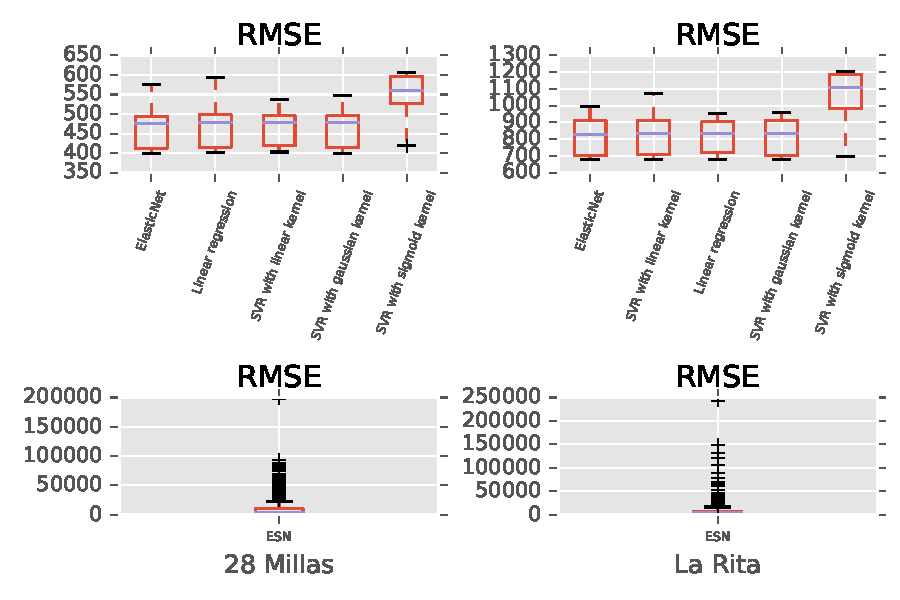
\includegraphics[scale=.8]{Usado_2017-04-30_Sigatoka_RMSE_Boxplot_4}
 \caption{Box plots de los RMSE para cada una de las Fincas} 
 \label{figura4} 
\end{figure}
%
\figref{figura5} shows the Pareto frontier for each farm with respect to $R^2$ and $RMSE$. La Rita obtains upper $R^2$ with respect to 28 Millas, but 28 Millas obtains better $RMSE$ than La Rita. This situation arise because $RMSE$ considers errors only with respect the prediction and in 28 Millas the average of Stage of Evolution is $4316.16$, unlike, in La Rita the average is $5507.30$. So, in La Rita we obtains higher errors in absolute values. $R^2$  is a relative metric between 0 thru 1 and it is less sensitive to absolute values.
%
\begin{figure}[H] 
 \centering
 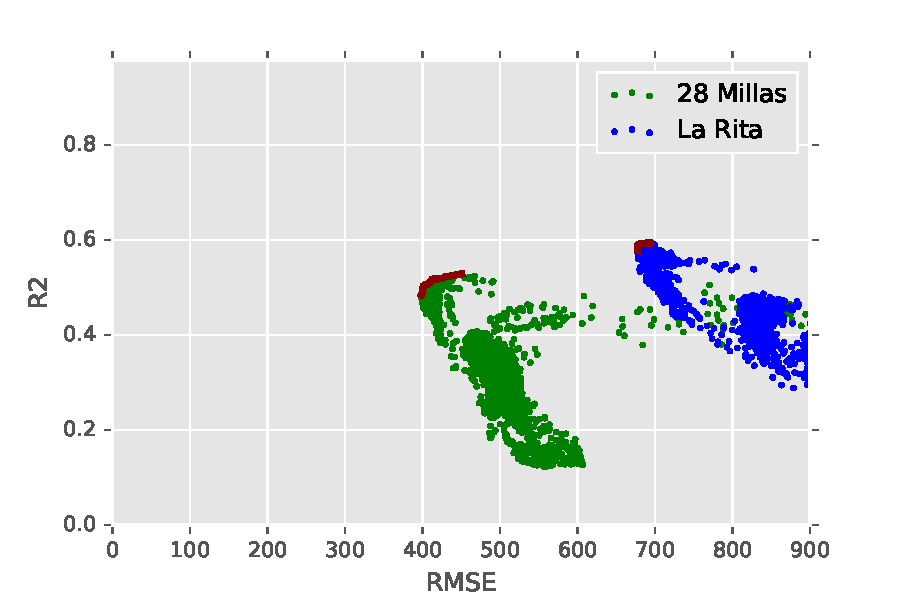
\includegraphics[scale=.8]{Usado_2017-04-30_Sigatoka_R2_RMSE}
 \caption{Pareto frontier for $R^2$ and $RMSE$} 
 \label{figura5} 
\end{figure}

The Pareto frontier for the La Rita farm is composed by 5 elements. The \tablename $.$\ref{tabla3} shows the composition about variables, observation ranges, techniques and weeks ahead.

\begin{table}[h] 
\caption{Composition of the Pareto frontier - La Rita} 
\label{tabla3} 
\centering
\begin{tabular}{c|c|c|c|c|c} 
\hline
\bfseries Variable & \bfseries Observation range & \bfseries Weeks ahead & \bfseries Technique &\bfseries $R^2$ & \bfseries $RMSE$\\ 
\hline\hline 
  &   &  &  &   &  \\



Pair $\overline{T}_{a}$ $\overline{W}$ &	1 to 1  & 36 & 64.25\% & 714.51 \\
 &	2 to 1  & 6 & 62.97\% & 695.10 \\
\hline 
All  & 1 to 1  & 18 & 62.98\% & 701.95 \\
   & 2 to 1  & 12 & 61.76\% & 679.92 \\
    & 3 to 1  & 6 & 60.60\% & 676.42 \\
    & 5 to 1  &  2 & 60.37\% & 672.39 \\
\hline    
$\overline{T}_{a}$ & 1 to 1  & 12  & 63.60\% & 708.77 \\
       &	2 to 1  & 4 & 62.23\% & 689.55 \\
\hline
\end{tabular} 
\end{table}

Similarly, the Pareto frontier for the 28 Millas farm is composed by 75 elements. The \tablename $.$\ref{tabla4} shows the composition about variables and observation ranges.

\begin{table}[h] 
\caption{Composition of the Pareto frontier - 28 Millas - Phase one} 
\label{tabla4} 
\centering
\begin{tabular}{c|c|c|c|c} 
\hline
\bfseries Variable & \bfseries Observation range & \bfseries Quantity & \bfseries Max $R^2$ & \bfseries Min $RMSE$\\ 
\hline\hline 
Pair $\overline{T}_{a}$ $\overline{W}$ & 1 to 1 & 8 & 57.80\% & 438.09 \\
\hline 
All   &	9 to 1 & 2 & 50.93\% & 397.93 \\
  & 10 to 1	 & 2 & 50.97\% & 398.81 \\
  &	8 to 1 & 6 & 51.62\% & 398.93 \\
  &	7 to 1 & 2 & 52.25\% & 400.28 \\
  &	6 to 1 & 2 & 53.16\% & 404.14 \\
  &	4 to 1 & 2 & 54.32\% & 407.54 \\
\hline    
$\overline{T}_{a}$ & 1 to 1  & 8  & 59.09\% & 439.44 \\
\hline
Pair $\overline{T}_{a}$ $\overline{H}$ & 1 to 1	 & 8 & 57.51\% & 428.61 \\
 &	2 to 1 & 20 & 56.91\% & 414.37 \\
 &	3 to 1 & 3 & 54.41\% & 411.55 \\
 &	4 to 1 & 3 & 53.34\% & 406.65 \\
\hline
Pair $\overline{T}_{a}$ $P$ & 3 to 1 & 9 & 56.23\% & 422.76 \\
\hline
\end{tabular} 
\end{table}



Now, the \figref{figura5} compares the mean of the $RMSE$ for each algorithm in the experiment, pero para la predicción de 1, 2 ó 3 semanas adelante con respecto a la información de las variables climatológocas y del preaviso biológico. Además, to predict one week ahead obtiene un RMSE más bajo que  two weeks ahead, and this is better than three weeks ahead. 
%
\begin{figure}[H] 
 \centering
 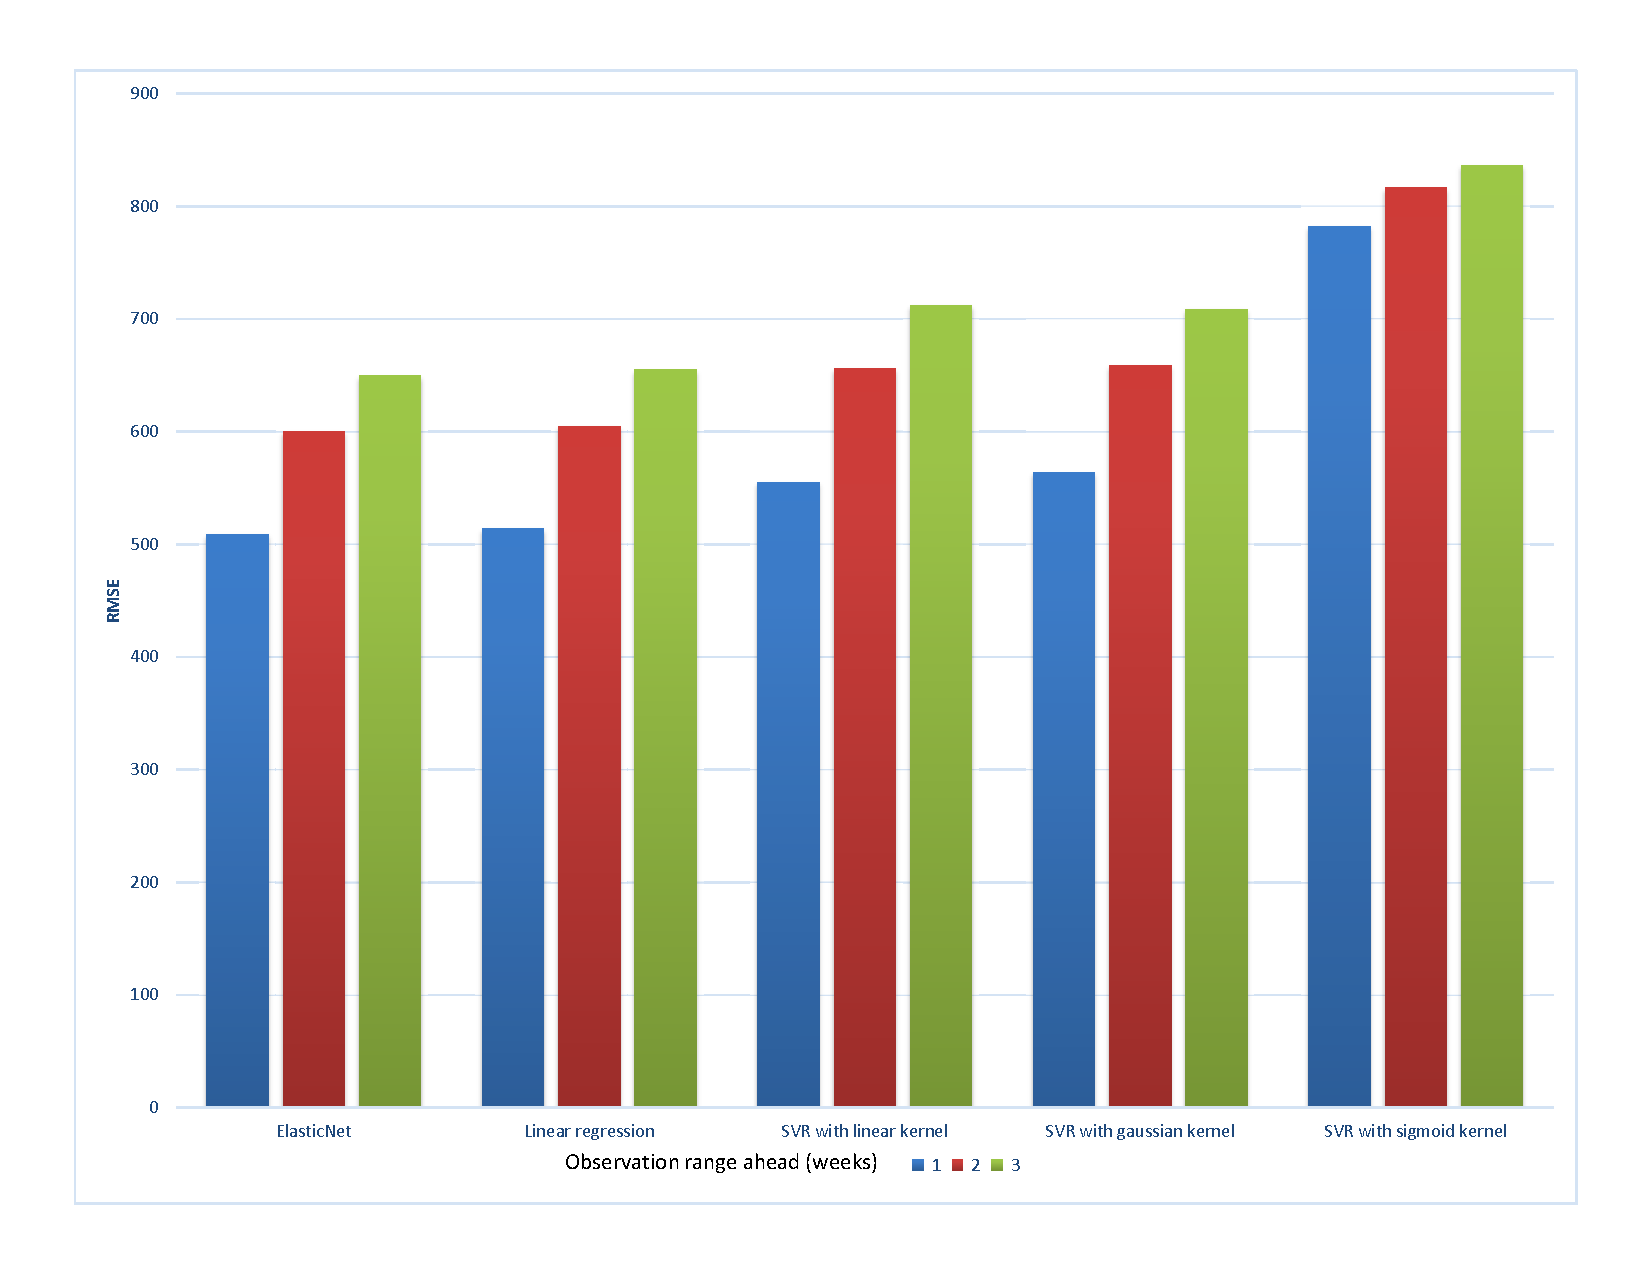
\includegraphics[scale=.5]{Usado_Algorithms-RMSE}
 \caption{$RMSE$ for each algorithm} 
 \label{figura5} 
\end{figure}

\figref{figura6} presents, for one, two and three weeks ahead, the best $R^2$. Results are group by farm. In general, to predict one week ahead is better than two weeks ahead and so on. The number of weeks consider in the observation range in the pattern is not the main discriminant factor, but it is clear that we get better $R^2$ for one week ahead than two weeks ahead and so on.

\begin{figure}[H] 
 \centering
 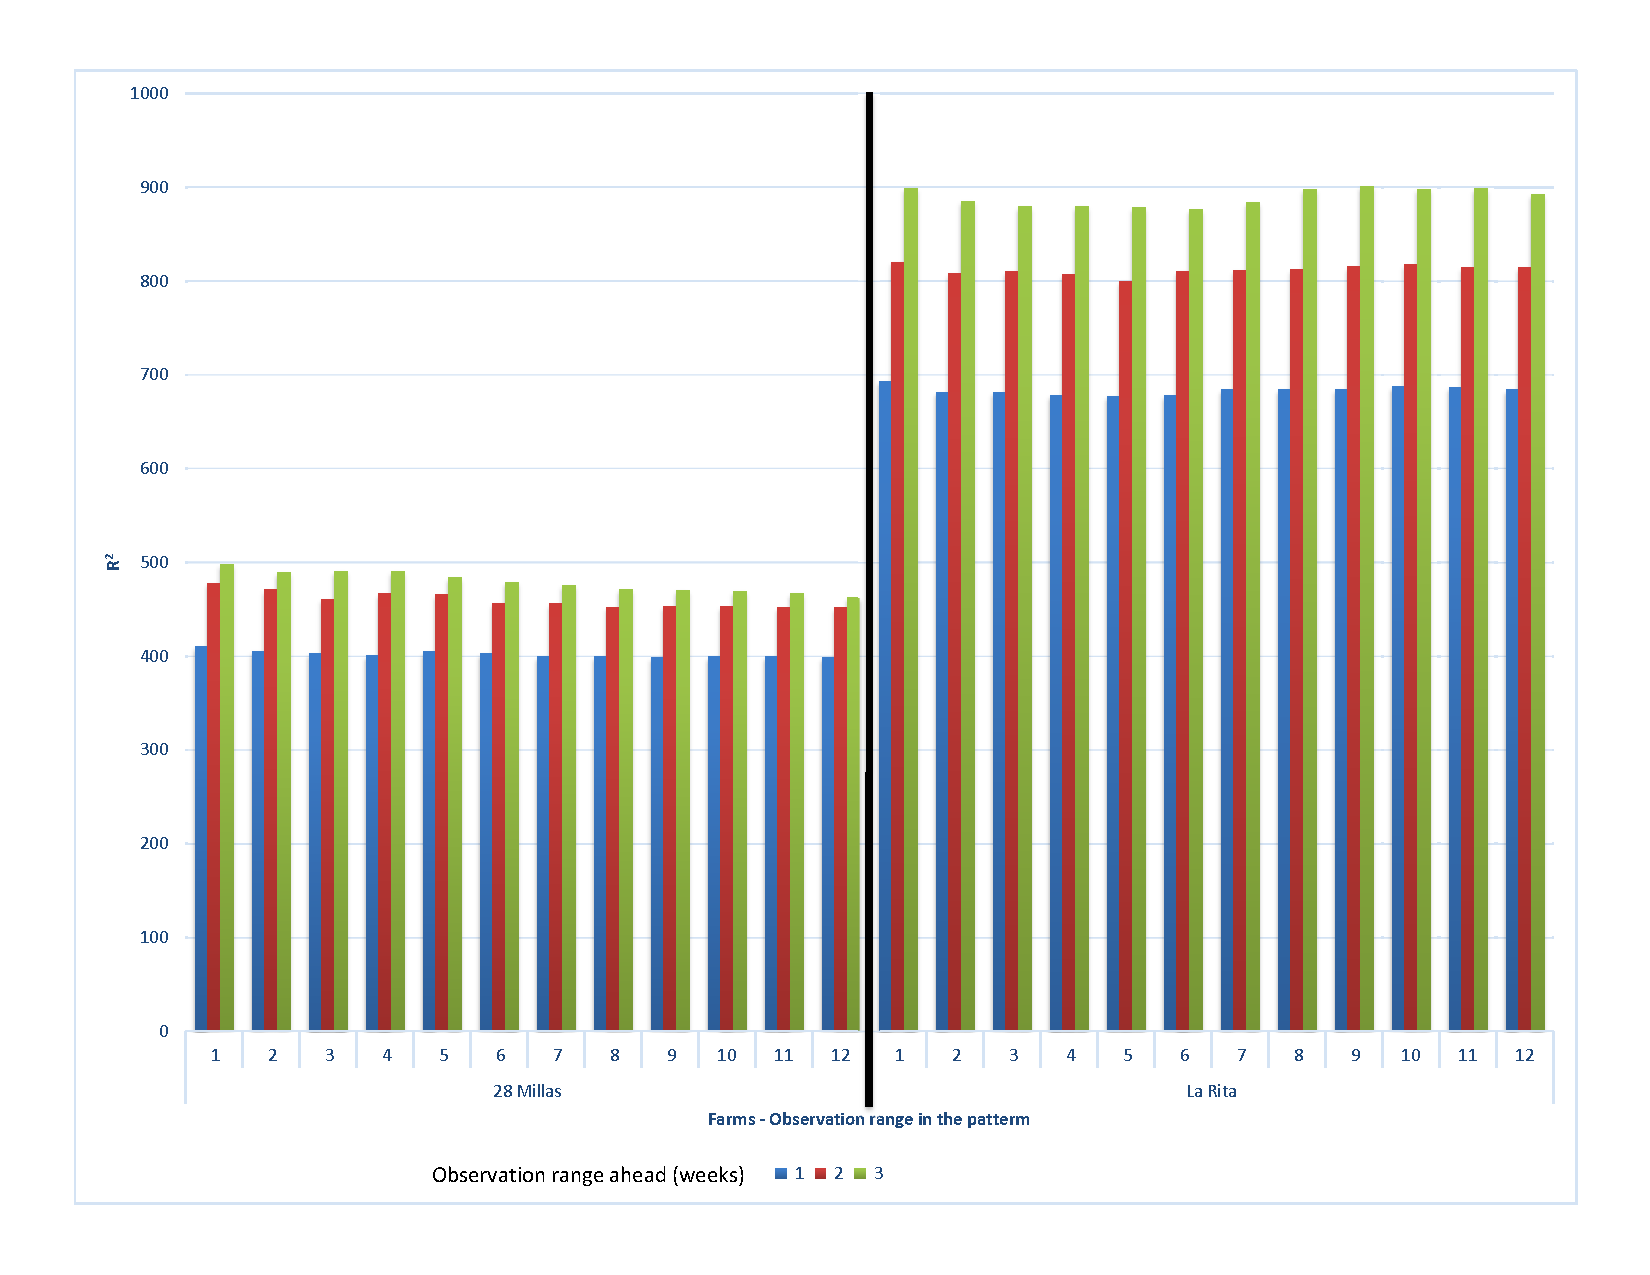
\includegraphics[scale=.5]{2017-01-15-Periods-R2}
 \caption{Phase one - Best $R^2$ for each observation range} 
 \label{figura6} 
\end{figure}

\figref{figura7} shows the best $R^2$ for each variables combination. Results are group by farm. The better results are obtained with $\overline{T}_{a}$ and the combination of $\overline{T}_{a}$ with $\overline{W}$, in both farms of similarly. You can note that the use of all variables in the model or the inclusion of the four variables suggest for expert criteria do not improve significantly the results, then the use of more sensors do not assure a better result. 

\begin{figure}[H] 
 \centering
 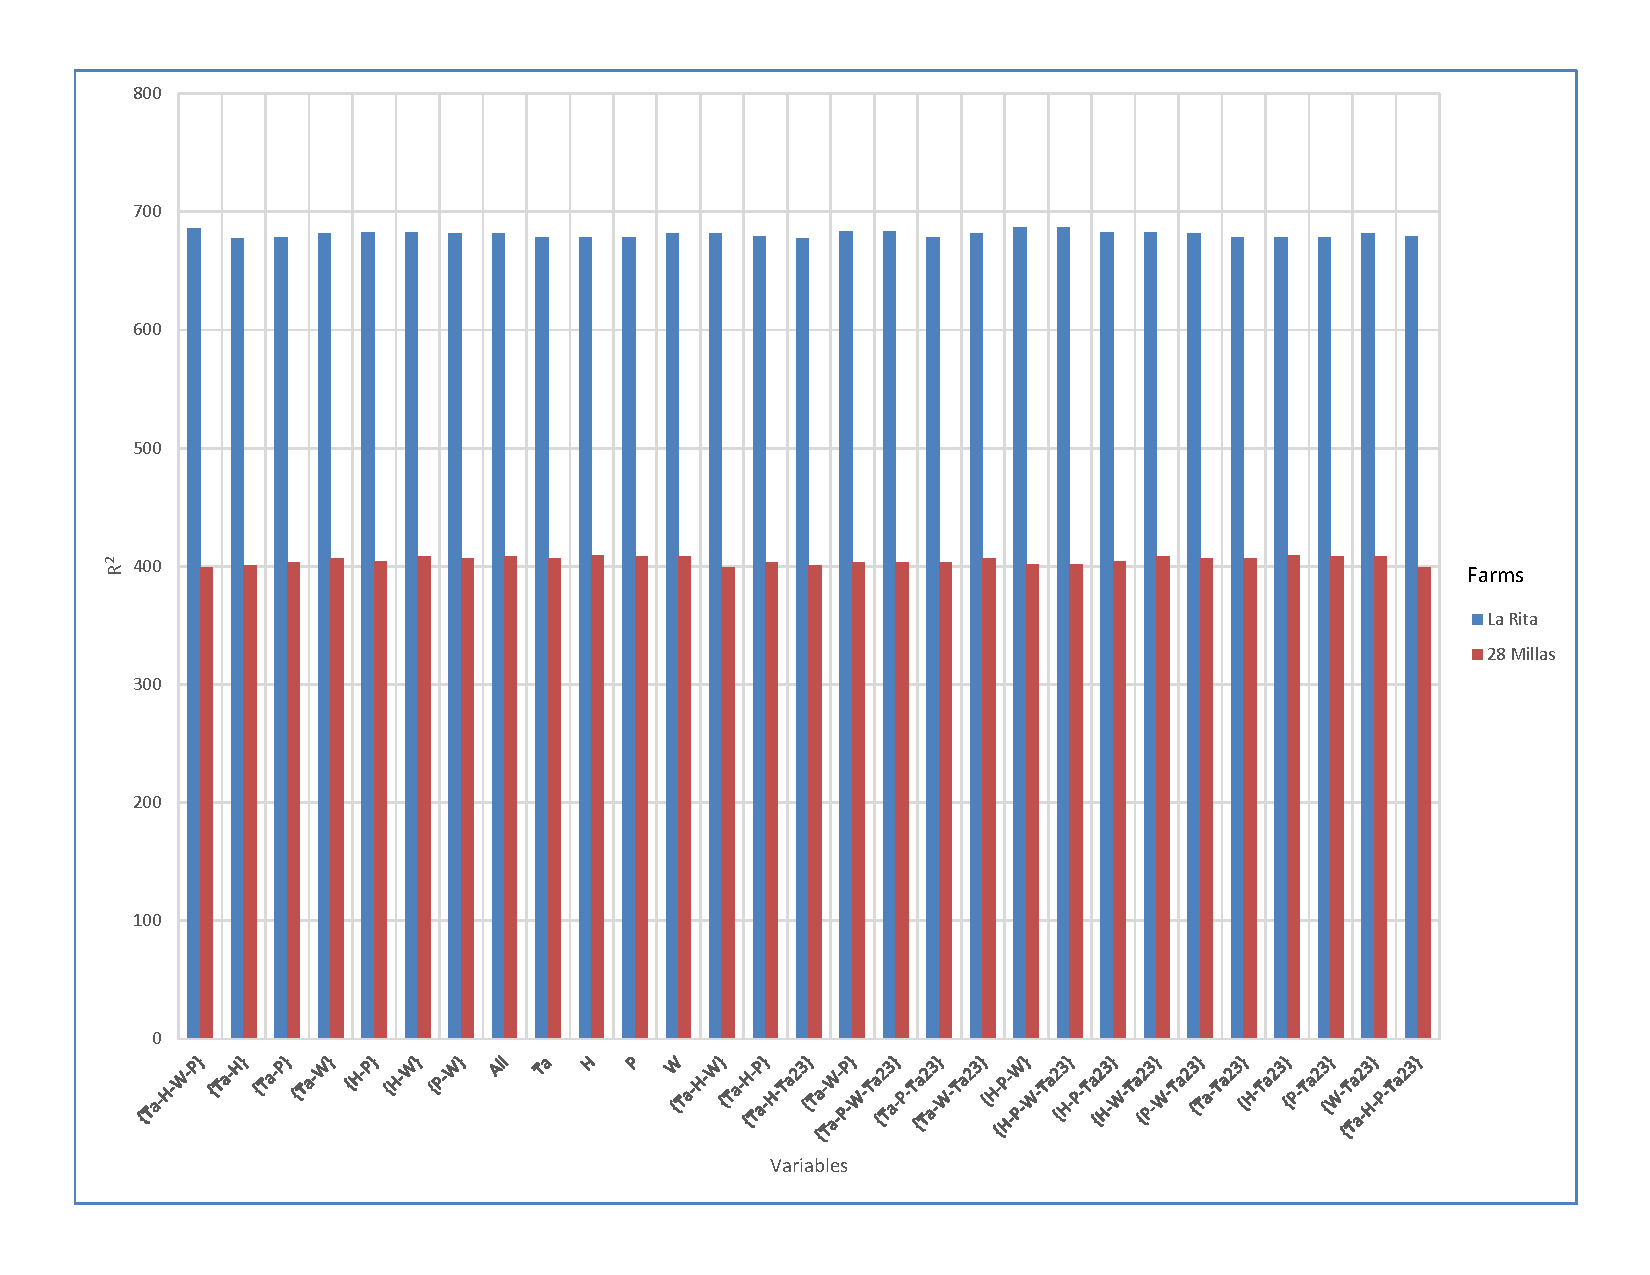
\includegraphics[scale=.5]{2017-01-15-Variables-R2}
 \caption{Phase one - Best $R^2$ for each variable combination} 
 \label{figura7} 
\end{figure}

We can conclude that the best configuration in both farms is to consider the climate and the evolution stage of the current week to predict the evolution stage of the next week.



\section{Conclusions and Future work}
Este estudio presentó la comparación de varias técnicas de machine learning en la predicción de la tasa de desarrollo de la enfermedad llamada Sigatoka negra. The following conclusions can be drawn:
\begin{enumerate}
\item Si bien los valores absolutos del $RMSE$ y el $R^2$ difieren entre las dos fincas en estudio, se mostró que al seleccopmar la técnica, la cantidad de semanas de observación, la cantidad de semanas hacia adelante a predecir y las variables a incluir en el modelo, coinciden los resultados. Lo cual es muestra de que estas características estan asociadas al fenómeno más que a una finca en particular.
\item Los menores $RMWE$ were reached with linear models.
\item  As little as three meteorological variables can be used because of the correlations detected among variables. 
\item Las ESN obtuvieron $RMWE$ muy altos, lo cual es producto de la cardinalidad del conjunto de datos, que no es suficiente para que la red neuronal se ajuste durante el entrenamiento.
\item Valores de $R^2$ cercanos al 60\% se alcanzaron en las pruebas.
\end{enumerate}
%
Future work of this research is focused on:
\begin{enumerate}
\item The extension of these findings to other farms.
\item The extension of the model to be applied in an early warning system, which does not require the regression task.
\item The use of image to increase the feature sets.
\end{enumerate}



\section*{Acknowledgements}

The authors would like to thank Corbana~S.\,A.\ for providing the data
for this research.

\section*{References}

\bibliography{references}

\end{document}